\chapter{Økonomi}
\section{Indledning}
I dette kapitel fokuseres på økonomiske aspekter ved erhvervelse af Appinux’ løsning til virtuel hjemmepleje, og der tages udgangspunkt i møder og emailkorrespondancer med henholdsvis Favrskov Kommune og Appinux. 

Økonomikapitlet har til formål at belyse omkostningerne ved henholdsvis fysisk hjemmepleje og virtuel hjemmepleje i Favrskov Kommune og derefter pointere økonomiske forskelle mellem de to scenarier ved hjælp af en ressourceopgørelse.

De økonomiske aspekter diskuteres, og afslutningsvis konkluderes der på udfaldet, hvorved det fokuserede spørgsmål besvares. 

\subsection{Fokuseret spørgsmål}
\begin{itemize}
	\item Hvilke økonomiske omkostninger er der ved implementering og drift af virtuel hjemmepleje med videoopkald sammenlignet med konventionel fysisk hjemmepleje i Favrskov Kommune?
\end{itemize}

\section{Metode}
Gennem møder med Appinux, Netplan Care og Favrskov Kommune er det nødvendige udstyr for at kunne implementere telesundhed – herunder virtuel hjemmepleje – blevet identificeret. 
Der er tilegnet informationer om diverse omkostninger ved dette udstyr samt yderligere omkring arbejdsgange i Favrskov Kommune.
På baggrund af sparsom information om specialaftalen indgået mellem Appinux og Favrskov Kommune, omfang af målgruppe og tidsbesparelser ved virtuel hjemmepleje sammenlignet med fysiske besøg er der opstillet en case herom. Casen og øvrige antagelser bygger på vejledende informationer fra Favrskov Kommune.

Yderligere økonomiske informationer er indsamlet gennem litteraturstudie. For en dybdegående beskrivelse af metoden henvises til \vref{chap:metode}. 

Specifikke emneord: \textit{Telemedicine, Telehealth, Telecare, Videoconference, Videoconferencing, Homecare, Elderly, Cost, Cost effectiveness, Video, Driving, Municipality.}
  


\section{Resultater}
Alle beregninger i resultatafsnittet er vedlagt som bilag [Bilag 15, 15.1]. 
\subsection{Omkostninger ved implementering og drift af Appinux' løsning}
\subsubsection{Opstartsomkostninger}
Opstartsomkostningerne for Appinux’ telesundhedsløsning med videoopkald ses på nedenstående figur 6.1. Der er vigtigt at pointere, at indkøb af tablets til selve videoopkaldende ikke er inddraget i figur 1, da den udelukkende belyser opstartsomkostningerne for Appinux’ løsning [Bilag 4, 4.1].

\begin{figure}[H]
	\centering
	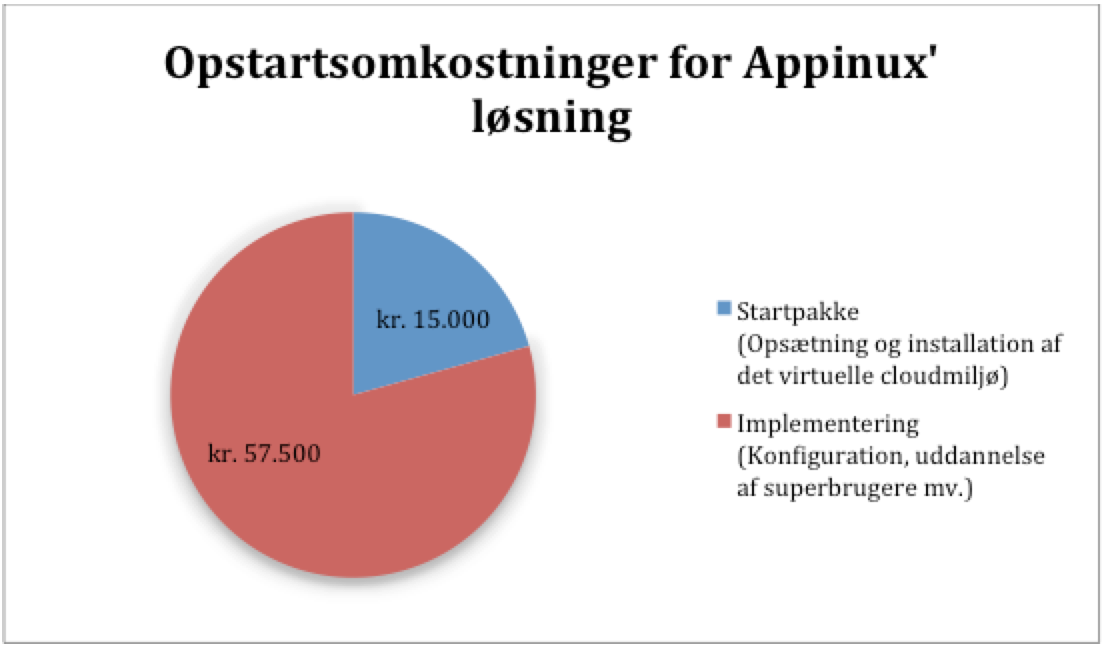
\includegraphics[width=1\textwidth]{Figurer/Skarmbillede_opstart}
	\caption{Opstartsomkostninger for videoopkald.}
\end{figure}

Appinux tilbyder ikke tablets som en del af løsningen, og det har ikke været muligt at indhente Appinux' anbefalinger til krav vedrørende tablets \vref{sec:implementeringsprocessen}.\\
Favrskov Kommune har informeret omkring indkøbet af tablets og covers til brug af netop Appinux’ løsning. \\
Tabel \ref{tab:tabelindkoeb} tager udgangspunkt i Favrskov Kommunes estimering om, at 25 tablets og covers er tilstrækkeligt med det nuværende potentiale for virtuel hjemmepleje. Prisen ses i tabel \ref{tab:tabelindkoeb} [Bilag 4, 4.1]. 

\begin{table}[H]
	\caption{Tabel over indkøb af tablets i Favrskov Kommune. [Bilag 15, 15.1]}
	\centering
	\label{tab:tabelindkoeb}
	\begin{tabular}{|l|l|l|l|}
		\hline
		\textbf{Beskrivelse} & \textbf{Pris} & \textbf{Antal} & \textbf{Samlet udgift}\\ \hline
		Samsung Tab A Tablet + cover & Kr. 2.300,00 pr. sæt & 25 stk. & kr. 57.500\\ \hline
	\end{tabular}
\end{table}
Det nødvendige antal tilgængelige tablets og covers vil afhænge af antallet af borgere. Udover borgerne skal de sundhedsprofessionelle ligeledes være i besiddelse af en tablet for at kunne foretage videoopkald til borgerne. \\
Favrskov Kommune antager, at der i fremtiden opstår behov for indkøb af flere nye tablets og covers, hvis der tages udgangspunkt i Favrskov Kommunes mål om at have 50 aktive brugere i form af borgere [Bilag 4, 4.1].

\subsection{Driftsøkonomi}
\subsubsection{Månedligt abonnement}
Favrskov Kommune abonnerer på Appinux’ løsning og betaler en månedlig pris for de tilkøbte moduler. Abonnementet varierer i pris alt efter, hvilke moduler der tilkøbes, og hvor mange brugere, der benytter modulet. \\
Der tages udgangspunkt i Appinux’ løsning for videoopkald (”Platform – Forløb, Kalender, Video”), da dette modul giver adgang til at anvende virtuel hjemmepleje [Bilag 9, 9.1]. Tabel \ref{tab:tabelmaanedudgift} skitser priserne for månedligt abonnement i forhold til antal brugere i form af borgere. 

\begin{table}[H]
	\caption{Tabellen skitserer de månedlige udgifter for modulet ”Platform – Forløb, Kalender, Video” alt efter antallet af brugere. Priserne er generelle og tager ikke højde for specialaftaler [Bilag 9, 9.1].}
	\centering
	\label{tab:tabelmaanedudgift}
	\begin{tabularx}{\textwidth}{|X|X|}
		\hline
		\textbf{Beskrivelse} & \textbf{Udgift}\\ \hline
		Månedligt abonnement ved Appinux 
		(0-75 brugere)
		 & Kr. 139,00 pr. bruger pr. måned\\ 
		\hline
		Månedligt abonnement ved Appinux 
		(76-300 brugere)
		& Kr. 119,00 pr. bruger pr. måned\\ \hline
				Månedligt abonnement ved Appinux 
				(0-500 brugere)
				& Kr. 22.500,00 pr. måned (Prisen er uafhængig af antallet af brugere, så længe det er mellem 0-500)\\ \hline
	\end{tabularx}
\end{table}

\subsubsection{Løn til personale}
Tabel \ref{tab:tabelpersonaleudgift} tager udgangspunkt i, at Sundhedscenter Hadsten vælger at opdatere systemet, hver gang Appinux stiller en opdatering til rådighed, hvilket er én gang i kvartalet. 

\begin{table}[H]
	\caption{Udgift for Favrskov Kommune for at lave systemopdateringer pr. år \cite{dsr}, [Bilag 15, 15.1].} 
	\centering
	\label{tab:tabelpersonaleudgift}
	\begin{tabularx}{\textwidth}{|X|X|}
		\hline
		Pris pr. år for at teste opdateringer
		& kr. 11.580,00\\ 
		\hline
	\end{tabularx}
\end{table}

Favrskov Kommune har dog mulighed for at fravælge hver anden opdatering og kun opdatere systemet én gang hvert halve år [Bilag 4, 4.1].

\subsubsection{Totalomkostninger}
Der tages ikke højde for løn til personale, der foretager videoopkald og sidder i call-center, uddannelse af superbrugere, forældede tablets, fejlkøb af tablets og en eventuel specialaftale mellem Favrskov Kommune og Appinux. Dette på baggrund af manglende information herom.

\begin{figure}[H]
	\centering
	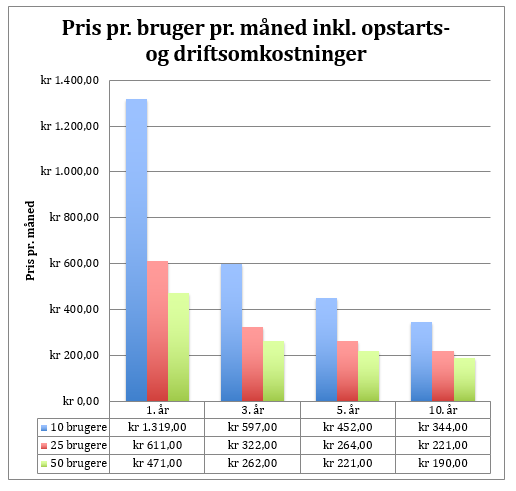
\includegraphics[width=0.9\textwidth]{Figurer/figuroko.png}
	\caption{\label{fig:oekokort}Kolonnerne viser den umiddelbare pris pr. bruger pr. måned inklusiv opstarts- og driftsomkostninger samt indkøb af tablets og covers.
		Ved 10 og 25 brugere er der medregnet indkøb af 25 tablets, mens der ved 50 brugere er medregnet indkøb af 50 tablets [Bilag 15, 15.1].}
\end{figure}

Det ses, at prisen pr. bruger pr. måned varierer efter længden af perioden Favrskov Kommune vælger at benytte videoopkald.
Det skyldes, at opstartsomkostninger forekommer som engangsbetaling, og dermed vil den gennemsnitlige pris pr. bruger pr. måned falde i takt med anvendelsesperioden. Figur \ref{fig:oekokort} viser desuden, at prisen falder med stigende antal af brugere.  

\subsection{Økonomiske usikkerheder og yderligere omkostninger}
Dette afsnit har til formål at belyse økonomiske usikkerheder og eventuelle fremtidige omkostninger. 

\subsubsection{Superbrugere}
Favrskov Kommune har i alt 26 superbrugere tilknyttet Appinux’ løsning, hvoraf nogle af dem er tilknyttet virtuel hjemmepleje. Superbrugere er sundhedsprofessionelle. For mere detaljeret beskrivelse af superbrugernes opgave, se \vref{sec:arbejdsgange}.   

Hvert halve år afholdes et fælles superbrugermøde af halvanden times varighed for alle superbrugere [Bilag 8, 8.5], hvilket ligeledes er en omkostning, der skal tages i betragtning ved erhvervelse af virtuel hjemmepleje. 

Det må antages, at kommunen skal bruge yderligere ressourcer på uddannelse af nye superbrugere i tilfælde af, at personale kvalificeret som superbruger fratræder sin stilling. \\
Omkostningen må forventes at variere i forbindelse med antallet af borgere, idet flere borgere kræver mere personale til håndtering af videoopkald [Bilag 11, 11.45].

\subsubsection{Tablets}
Favrskov Kommune købte - ved starten af samarbejdet med Appinux - nogle nye tablets, men de tekniske kvalifikationer var ikke tilstrækkelige til at benytte videoopkald, hvorfor efterfølgende indkøb af bedre tablets var nødvendigt. Se \vref{sec:implementeringsprocessen}.  \\
I fremtiden kan der opstå behov for yderligere indkøb af tablets i tilfælde af, at antal brugere overstiger antallet af indkøbte tablets. Ydermere kan ekstra indkøb af tablets forekomme som resultat af defekte tablets.

\subsubsection{Antal brugere}
Figur \ref{fig:oekokort} viser, at prisen falder med stigende antal af brugere. Omfanget af brugergruppen har derfor stor betydning for de økonomiske konsekvenser. 

\subsubsection{Ugennemsigtige priser}
Priserne er bygget på listepriser fra Appinux samt informationer og antagelser fra Favrskov Kommune og bygger ikke på den reelle pris indgået mellem Favrskov Kommune og Appinux [Bilag 4, 4.1].  

\subsection{Omkostninger ved fysiske besøg}
\subsubsection{Transportomkostninger og løn til personale}
Med udgangspunkt i kørelisten [Bilag 8, 8.1] udleveret af Favrskov Kommune og en antaget gennemsnitlig køreafstand mellem hver borger på 5 km samt statens takst på 3,63 kr./km er transportomkostningen pr. fysisk besøg udregnet [Bilag 11, 11.45].\\
Endvidere er arbejdstimer udregnet med udgangspunkt i Favrskov Kommunes estimerede varighed af et fysisk besøg til Medicingivning på 10 minutter [Bilag 4, 4.1], se tabel \ref{tab:tabelfysiskbes}.

\begin{table}[H]
	\caption{Tabellen viser pris pr. fysisk besøg (Medicingivning) [Bilag 15, 15.1]}
	\centering
	\label{tab:tabelfysiskbes}
	\begin{tabular}{|l|l|l|l|}
		\hline
		\textbf{Transportomkostninger} & \textbf{Arbejdstimer } & \textbf{Arbejdsløn \cite{foa}} & \textbf{I alt pr. besøg}\\ \hline
		kr. 18,15 & 0,1667 & kr. 22,58 & kr. 40,73\\ \hline
	\end{tabular}
\end{table}


\subsection{Ressourceopgørelse}
Det forventes, at videoopkaldene vil reducere arbejdstiden pr. besøg inklusiv transport fra ti til tre minutter [Bilag 4, 4.1], hvilket ses i tabel \ref{tab:tabelbesparelse}.

\begin{table}[H]
	\caption{Tabellen viser besparelsen pr. virtuelt besøg i forhold til fysisk besøg (eksklusiv opstarts- og driftsomkostninger) [Bilag 15, 15.1].}
	\centering
	\label{tab:tabelbesparelse}
	\begin{tabular}{|l|l|l|l|}
		\hline
		\textbf{Transportomkostninger} & \textbf{Arbejdstimer } & \textbf{Arbejdsløn \cite{foa}} & \textbf{I alt pr. besøg}\\ \hline
		kr. 18,15 & 0,1667 & kr. 15,80 & kr. 33,95\\ \hline
	\end{tabular}
\end{table}

Der tages udgangspunkt i ydelsen Medicingivning, hvor sundhedsprofessionelle har mellem en og fire besøg pr. dag pr. borger. Her er videoopkaldene estimeret til at kunne erstatte en til to af de fysiske besøg. Favrskov Kommune kan dog ikke sige med sikkerhed, i hvor stort omfang fysiske besøg vil blive erstattet af videoopkald. Favrskov Kommune estimerer alt mellem et besøg pr. uge til flere om dagen [Bilag 11, 11.45], hvilket giver anledning til at kigge på det nødvendige antal besøg pr. borger pr. måned før implementering af videoopkald medfører økonomisk gevinst.\\
Tallene er udregnet efter prisen pr. borger, se figur \ref{fig:oekokort}.

\begin{table}[H]
	\caption{Tabellen viser det minimale antal af besøg pr. bruger pr. måned, for at videoopkald via virtuel hjemmepleje bliver rentabelt i forhold til fysiske besøg [Bilag 15, 15.1].}
	\centering
	\label{tab:tabelminimum}
	\begin{tabular}{|l|l|l|l|l|}
		\hline
		 & \textbf{1 år} & \textbf{3 år} & \textbf{5 år} & \textbf{10 år}\\ \hline
		\textbf{10 brugere} & 39 & 18 & 14 & 11\\ \hline
		\textbf{25 brugere} & 18 & 10 & 8 & 7\\ \hline
		\textbf{50 brugere} & 14 & 8 & 7 & 6\\ \hline
	\end{tabular}
\end{table}

\section{Diskussion}
Med udgangspunkt i ovenstående ressourceopgørelse kan indførelse af virtuel hjemmepleje i Favrskov Kommune medføre både positive og negative økonomiske konsekvenser alt efter, hvordan de forskellige variable omkostninger forholder sig. 


På kort sigt vil opstartsomkostningerne sandsynligvis bevirke et underskud for virtuel hjemmepleje i forhold til de fysiske besøg, hvor prisen pr. bruger pr. måned er høj sammenlignet med prisen efter for eksempel 10 år. Det systematiske review \citetitle{jose} konkluderede hertil, at de langsigtede omkostninger og gevinster er vigtige, da besparelser ved videoopkald muligvis først kommer til syne på lang sigt \cite{jose}. Men her er det nødvendigt at være opmærksom på, at Favrskov Kommune har lavet en specialaftale med Appinux, hvorved opstartsomkostningerne og den månedlige betaling pr. bruger muligvis er lavere end antaget i ressourceopgørelsen [Bilag 4, 4.1]. 


Den månedlige pris pr. bruger kan falde, hvis antallet af brugere overskrider 75, se tabel \ref{tab:tabelmaanedudgift}. Med udgangspunkt i Sundhedscenter Hadstens forventninger til fremtidige antal brugere [Bilag 4, 4.1] bør denne besparelse dog ikke inddrages som en forventelig minimering af driftsomkostningerne. 
Favrskov Kommune kan derimod hente besparelser på driftsomkostningerne i form af nedskæringer i antallet af opdateringer, der stilles til rådighed fra Appinux. Kommunen har mulighed for at skære fra fire årlige opdateringer til to, hvorved det er muligt at holde driftomkostningerne nede til et minimum [Bilag 4, 4.1].
Modsat bør det nævnes, at Favrskov Kommune vil opleve yderligere udgifter i fremtiden, såfremt de ønsker ny- eller videreuddannelse af superbrugere samt i tilfælde af defekte tablets.  
Der skal desuden tages højde for, at ressourceopgørelsen ikke inkluderer arbejdstimer i call-centeret, hvor de to hovedeansvarlige for \textit{Pilotprojekt Videokommunikation} har ansvaret for alt vedrørende Appinux, herunder implementering, undervisning og support på både anvendelse og tekniske problemer [Bilag 8, 8.5].

Der stilles spørgsmålstegn ved den forventede tid, der spares pr. videoopkald ved virtuelle besøg kontra fysiske besøg, idet beregninger er lavet på baggrund af estimeringer fra Sundhedscenter Hadsten. I \textit{Pilotprojekt Videokommunikation} var tidsbesparelsen mindre end forventet på baggrund af tekniske udfordringer ved videoopkald [Bilag 4, 4.1]. 
I modsætning hertil viser et deskriptivt, retrospektivt studie \citetitle{solrun}, at kørselstiden underestimeres ved fysiske besøg \cite{solrun}. Dog vides det ikke præcist, hvor meget tid, der spares ved videoopkald kontra fysiske besøg.

Den største faktor vedrørende de økonomiske konsekvenser for virtuel hjemmepleje sammenlignet med fysiske besøg er antallet af besøg pr. borger. Det vil være økonomisk fordelagtigt at foretage mange videoopkald for et lille antal brugere, hvorimod et lavt antal videoopkald for mange brugere sandsynligvis vil have en negativ økonomisk konsekvens. 
Ifølge pilotstudiet \citetitle{cost} er netop antallet af besøg altafgørende, hvis der skal findes økonomisk gevinst ved videoopkald som erstatning for fysiske besøg \cite{cost}. 


\section{Delkonklusion}
Opstartsomkostningerne ved implementering af Appinux’ løsning med videoopkald er relativt stor, hvilket bevirker en negativ økonomisk konsekvens på kort sigt. 
Overordnet set vil mange variabler have betydning for den økonomiske konsekvens på både kort og lang sigt, hvor blandt andet antal opdateringer kan minimeres med henblik på besparelser. 
Potentialet for økonomisk gevinst afhænger i høj grad af antallet af fysiske besøg, der erstattes pr. borger pr. måned, da der her foreligger besparelser på henholdsvis transportomkostninger og arbejdstid.
På lang sigt vil der være grundlag for økonomisk gevinst ved implementering af Appinux’ telesundhedsløsning med videoopkald, men det kræver, at Favrskov Kommune formår at erstatte et tilstrækkeligt antal fysiske besøg pr. borger pr. måned med videoopkald.






